The following sections are dedicated to the Wireless Communications Layer of this project. This layer includes the Ethernet Subsystem and the Black Box Subsystem. The Wireless Communications Layer manages the communications demands between the Web Interface Layer and the Camera Layer via UDP transport protocol over a wireless network provided the consumer by TrafficNet LLC.

\subsection{Black Box Subsystem}

\begin{figure}[h!]
	\centering
 	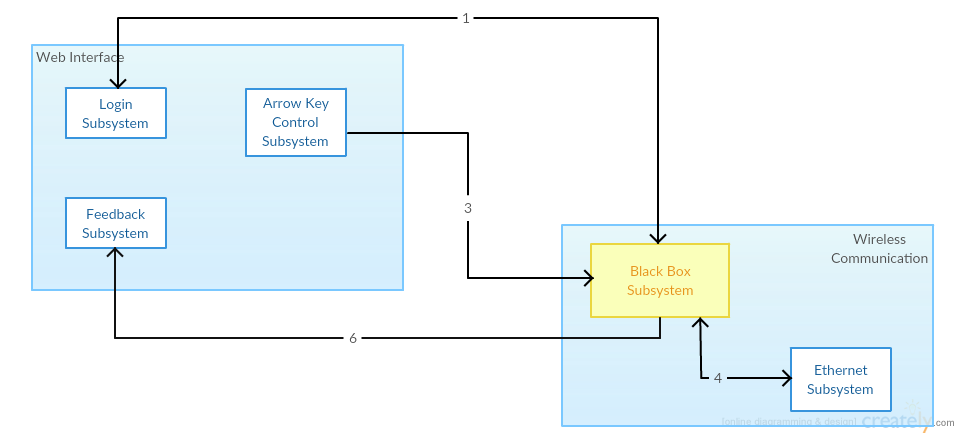
\includegraphics[width=0.60\textwidth]{images/ADSdiagrams/blackboxsubsystem.png}
 \caption{Black Box description diagram}
\end{figure}

The above diagram illustrates graphically the interaction of the Black Box Subsystem with other Subsystems from the Web Interface Layer. 

\subsubsection{Assumptions}
The Black Box Subsystem is one of two Subsystems that is necessary for this Architectural Design Specification but is provided entirely by TrafficNet LLC. Therefore it is assumed to be the responsibility of the vendor to provide.

\subsubsection{Responsibilities}
The Black Box provides the secure wireless communication between the Web based UI and the Raspberry Pi housed within the Camera. ZeroMQ establishes a TCP transfer protocol over a wireless network provided by the Black Box that may be accessed only by authorized users from a directly linked host machine. Authorized users may then use this network to send control signals from the host machine through the wireless network to the Raspberry Pi, as well as receive video feedback through the wireless network provided by the Black Box.

\subsubsection{Subsystem Interfaces}

\begin {table}[H]
\caption {Subsystem interfaces} 
\begin{center}
    \begin{tabular}{ | p{1cm} | p{6cm} | p{3cm} | p{3cm} |}
    \hline
    ID & Description & Inputs & Outputs \\ \hline
    \#1, 3, 4, 6 & Interaction between Black Box and the Web Interface/bus & \pbox{3cm}{Login server \\ Arrow Key Control \\ Ethernet} & \pbox{3cm}{Video Feedback \\ Login validation \\ TCP segments}  \\ \hline
    \end{tabular}
\end{center}
\end{table}

\subsection{Ethernet Subsystem}

\begin{figure}[h!]
	\centering
 	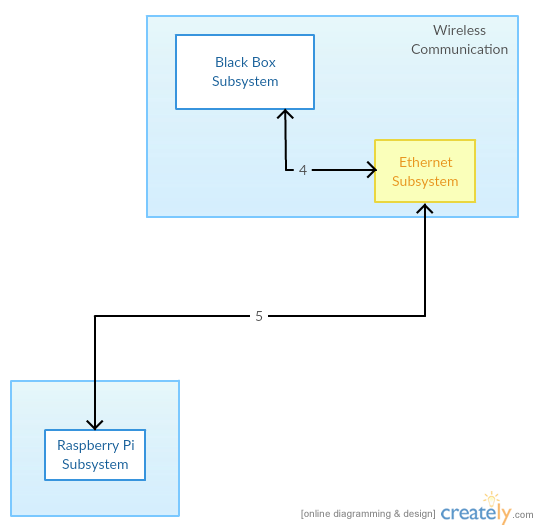
\includegraphics[width=0.60\textwidth]{images/ADSdiagrams/ethernetsubsystem.png}
 \caption{Ethernet description diagram}
\end{figure}

The above diagram illustrates graphically the interaction between the Ethernet Subsystem, the Black Box Subsystem, and the Raspberry Pi Subsystem of the Camera Layer. 

\subsubsection{Assumptions}
The Ethernet Subsystem is the physical connection between the Black Box Subsystem and the Raspberry Pi Subsystem of the Camera Layer.

\subsubsection{Responsibilities}
The Ethernet Subsystem is responsible for providing a physical link between the Black Box provided by TrafficNet LLC and the Raspberry Pi. It is the point at which wireless commands are physically recieved by the Camera Layer from the Wireless Communications Layer, and sent in the form of video feedback through the wireless network.

\subsubsection{Subsystem Interfaces}

\begin {table}[H]
\caption {Subsystem interfaces} 
\begin{center}
    \begin{tabular}{ | p{1cm} | p{6cm} | p{3cm} | p{3cm} |}
    \hline
    ID & Description & Inputs & Outputs \\ \hline
    \#4, 5 & Interaction between Raspberry Pi and the Ethernet/bus & \pbox{3cm}{Black Box Wireless Commands \\ Raspberry Pi TCP Communication} & \pbox{3cm}{Video Feedback \\ Login validation \\ TCP segments}  \\ \hline
    \end{tabular}
\end{center}
\end{table}
